\documentclass[a4paper]{article}


\usepackage[margin=1in]{geometry} % full-width

% AMS Packages
\usepackage{amsmath}
\usepackage{amsthm}
\usepackage{amssymb}

% Unicode
\usepackage[utf8]{inputenc}
\usepackage{hyperref}
\hypersetup{
	unicode,
	pdfauthor={María San José Seco},
	pdftitle={Estudio práctico de técnicas de ofuscación y contramedidas aplicables},
	pdfsubject={Estudio práctico de técnicas de ofuscación y contramedidas aplicables},
	pdfkeywords={obfuscation, malware, javascript},
	pdfproducer={María San José},
	pdfcreator={María San José}
}


% Natbib
\usepackage[sort&compress,numbers,square]{natbib}
\bibliographystyle{mplainnat}


\usepackage{graphicx, color}
\graphicspath{{fig/}}

\usepackage[spanish]{babel}

\usepackage{algorithm, algpseudocode} % use algorithm and algorithmicx for typesetting algorithms
\usepackage{mathrsfs} % for \mathscr command

\usepackage{lipsum}

\usepackage{fancyhdr}
\pagestyle{fancy}
\fancyhead{} % clear all header fields
\fancyhead[R]{\textbf{TFM: Estudio práctico de técnicas de ofuscación y contramedidas aplicables}}
\fancyfoot{} % clear all footer fields
\fancyfoot[R]{\thepage}

% Author info
\title{Estudio práctico de técnicas de ofuscación y contramedidas aplicables}
\author{María San José Seco \\ \href{https://github.com/drkrysSrng/freyja}{@drkrysSrng/freyja}}

\date{
	Universidad Católica de Murcia \\
	ENIIT - Campus Internacional de Ciberseguridad
}

\begin{document}

	\maketitle
	
	\begin{abstract}
		
	A lo largo de la historia, tanto como para proteger la propiedad intelectual o intercambiar secretos, se ha utilizado la ofuscación como medida de protección. El malware la ido evolucionando a través de los años utilizando diferentes técnicas cada vez más avanzadas de manera que los antivirus y los analistas no puedan detectarlos y evadirlos, ya que este método previene los análisis por firma o hash o por las reglas YARA que ayudan a buscar cadenas de texto sospechosas dentro de ellos. 
	\end{abstract}
	
	\section{Tipos de ofuscación}
	
	Hay varios tipos de ofuscación, que han ido evolucionando a través de la historia. Éstos son:
	
	\begin{itemize}
		\item \textbf{Packing:} Para cambiar la firma del malware malicioso, se comprime y se empaqueta dentro de otro ejecutable y sólo se desempaqueta cuando se va a ejecutar.
		\item \textbf{Inserción de código basura:} Dentro del código se inserta código que no tiene ninguna funcionalidad, lo que hace cambiar la firma del binario final.
		\item \textbf{XOR:} Esta operación booleana es conocida debido a que se utiliza tanto como para ofuscar commo para encriptar, ya que su utilización es sencilla. Basándonos en que un número xoreado consigo mismo nos da 0, podemos utilizar éstas instrucciones para modificar el código, recuperando el valor inicial de los parámetros fácilmente.
		\item \textbf{Reasignamiento de registros:} Simplemente se hacen copias de los parámetros sin afectar al programa final.
		\item \textbf{Sustitución de instrucciones:} Esta forma permite reemplazar operaciones que tiene el malware origial, por otras que aunque sean más lentas, cambiar la firma y dificultan el trabajo del analista.
		\item \textbf{Base64:} Muy utilizado para ocultar cadenas de texto como por ejemplo las URLs donde se conecta el malware.
		\item \textbf{Transposición de código:} Se cambian las instrucciones de lugar o se crea nuevo código para añadir más instrucciones y poder reordenar las originales.
		\item \textbf{Integración de código:} Hay malware que es capaz de infectar otros archivos del sistema o binarios commo si fuese un parásito para que cuando éstos se ejecuten, se ejecute la infección.
		\item \textbf{Expreciones MBA:} Sirven para ofuscar el código utilizando poliomios y operadores booleanos para sustituirlo por operaciones equivalentes sin alterar el valor de los parámetros.
		\item \textbf{Expresiones Opacas:} Son expresiones cuyo valor es Verdadero o Falso siempre pero que su valor no se obtiene hasta que no se esté ejecutando el malware.
		
	\end{itemize}


	\section{Enriptación, Compresión y Metamorfismo}
	
	El metamorfismo es lo que nos encontramos hoy en día, ya que se ha avanzado mucho para evadir los antivirus. De esta manera, la evolución del malware parte desde el punto de encontrarnos muestras oligomórficas, donde la parte viral está encriptada, muestras polimórficas, donde no soĺo está encriptado sino que también está ofuscado. El primer malware polimórfico de la Historia, Luna fue desarrollado en España por Bumblebee en el año 1999. 
	
	Finalmente los malware han evolucionado a malware de tipo metamórfico, de este modo, no nos encontraremos dos muestras iguales, ya que su ofuscación tiene muchas variaciones para reordenar las subrutinas.
	
	Para ello, el elemento más importante en este último caso es el motor metamórfico, que es el responsable de hacer todas las operaciones de evasión.
	
	\section{Análisis Entropía}
	Claude E. Shannon en \textit{A Mathematical Theory of Communication} desarrolló una fórmula donde, se puede identificar la aleatoriedad o desorden de un sistema, de manera que podamos identificar si una muestra ha sido ofuscada o no. Cuanto más alta sea la probabilidad y sobre todo mayor de \textit{3.75} significa que no ha sido escrito por un humano.
	
	\section{Importancia de las amenazas de JavaScript en Windows}
	Los ataques basados en script se han convertido en una amenaza importante en los últimos años. Siendo el 40\% de los últimos años, entre los lenguajes más utilizados se encuentran PowerShell, VBScript y JavaScript. Sin embargo la mayoría de malware se están migrando a éste último ya que es un lenguaje que se puede ejecutar dentro y fuera del navegador.
	
	\section{Desofuscación de código en JavaScript}
	Las técnicas más utilizadas de ofuscación en el malware que utiliza JavaScript son:
	\begin{itemize}
		\item Nos podemos encontrar todo el código en una sola línea.
		\item Uso de funciones con llamada instantánea tipo \verb*|(function hello(){})()|
		\item Concatenación de caracteres, conjuntos de caracteres, uso de \verb*|parseInt| y \verb*|toString| para sustituir un caracter por su valor equivalente.
		\item Llamar a funciones con cadenas de caracteres.
		\item Operadores lógicos equivalentes tipo \verb*|+!!false| que es 0
		\item Función \verb*|eval| con conjuntos de números
		\item Uso de caracteres Unicode, hexadecimal y formato URL
		\item Base64 para ocultar cadenas de caracteres como URLs	
	\end{itemize}
	
	\section{Freyja Deobfuscation Tool }
	\href{https://github.com/drkrysSrng/freyja}{@drkrysSrng/freyja}
	
	Se ha desarrollado la siguiente herramienta para aplicar varios tipos de ofuscación mencionados en el apartado anterior:
	
	\begin{itemize}
		\item Limpia el código y lo tabula de manera similar, no sólo tabulando las instrucciones, sino que parsea los caracteres en hexadecimal y unicode.
		\item Chequeeo de la entropía con el algoritmo de Shannon, línea por línea o por texto completo.
		\item Cuando los caracteres Unicode o en Hexadecimal no están parseados ya que no están en formato String sino que es una variable ofuscada, se parsean a mayores también.
		\item Desofusca funciones como \verb*|toString|, conjuntos de números dentro de \verb*|eval|, sustituir \verb*|unescape| y \verb*|parseint|:
		\item Concatena cadenas de caracteres separadas con el símbolo \verb*|+|
		\item Búsqueda de strings en base64 y su decodificación.
	\end{itemize}

	\begin{figure}[H]
		\centering
		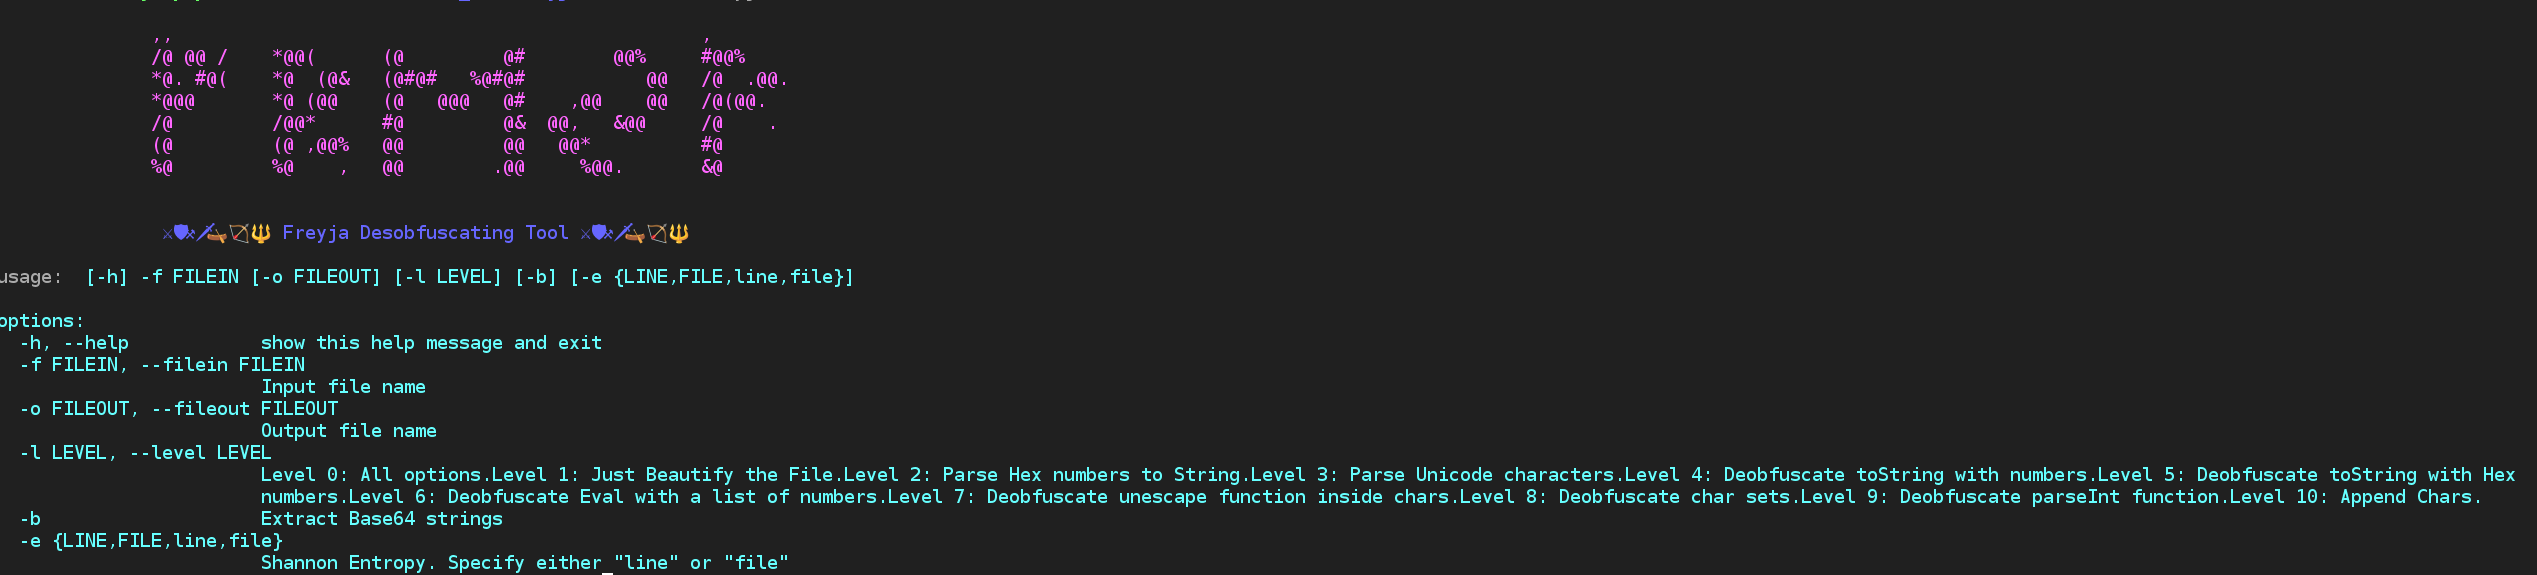
\includegraphics[width=18cm]{images/usage.png}
	\end{figure}
\end{document}

